\vspace{-10pt}
\section{Experiments}

%We conducted extensive ablation studies to evaluate the contribution of each component of our proposed method. We emphasize validation loss for model selection due to the relatively small validation set size (180 videos), which can make accuracy metrics noisy.

Extensive ablation studies were conducted to evaluate the contribution of each component of the proposed method.
The emphasis placed on validation loss for model selection is due to the relatively small size of the validation set (180 videos), which can render accuracy metrics unreliable.

\subsection{Implementation Details}

%For our proposed model, we utilized a Multi-Layer Perceptron (MLP) architecture. The input to the MLP was formed by concatenating pre-extracted video, audio (from TwelveLabs models), and string metadata embeddings (from OpenAI models). Based on our ablation studies, the optimal architecture was a 4-layer MLP with Swish~\cite{hendrycks2016gaussian} activation functions, dropout layer and batch normalization layer in the hidden layers and a final softmax layer for classification across the 10 categories.

%The model was trained for 20 epochs with a batch size of 8. We employed the AdamW~\cite{loshchilov2017decoupled} optimizer and a Cosine Annealing learning rate scheduler with a peak learning rate of $1\times 10^{-4}$ and a linear warm-up period of 1 epoch. The standard cross-entropy loss function was used for training. Data augmentation, with a strength of 0.5 as determined by our ablation studies, was applied to the input embeddings during training.

For the proposed model, an MLP architecture was utilized.
The input was formed by concatenating pre-extracted video, audio (from TwelveLabs models), and string metadata embeddings (from OpenAI models).
Considering the findings from the ablation experiments, it can be concluded that the most effective architecture is a 4-layer MLP with Swish ~\cite{hendrycks2016gaussian} activation functions, a dropout layer, batch normalization layers within the hidden layers and a final softmax layer, for the classification across the 10 distinct categories.
The model was trained over a period of 20 epochs, with a batch size of 8.
The AdamW ~\cite{loshchilov2017decoupled} optimizer and a Cosine Annealing learning rate scheduler with a peak learning rate of $1\times 10^{-4}$ and a linear warm-up period of 1 epoch were employed.
The standard cross-entropy loss function was utilized for the training process.
The augmentation of data, with a strength of 0.5 as determined by our ablation studies, was applied to the input embeddings during the training process.

\subsection{Ablation Studies}

\subsubsection{Input Features}

%Our ablation study on input features revealed clear benefits to incorporating multimodal information alongside basic video embeddings. While adding audio embeddings to the video embeddings offered a modest performance increase, the inclusion of metadata embeddings provided the most substantial improvement in validation accuracy. Interestingly, combining all three embedding types (video, audio, and metadata) did not yield the best accuracy and also showed signs of potential overfitting, as indicated by its validation loss trend. Considering both the significant accuracy uplift and a stable validation loss profile, the combination of video and metadata embeddings emerged as the most effective and was selected for subsequent experiments.

This study has revealed the clear benefits of incorporating multimodal information alongside basic video embeddings.
While the incorporation of audio embeddings into the video embeddings resulted in a modest enhancement to performance, the integration of metadata embeddings yielded the most substantial enhancement in validation accuracy.
It is interesting to note that combining all three embedding types (video, audio, and metadata) did not result in the optimal level of accuracy and exhibited signs of potential overfitting, as indicated by its validation loss trend.
Based on a comprehensive evaluation encompassing both the substantial enhancement in accuracy and the consistent stability of validation loss profiles, the integration of video and metadata embeddings was identified as the most effective approach.
Consequently, this combination was selected for further experiments.

\begin{table}[hbt!]
\centering
\caption{Ablation Study on Input Features. Validation accuracy is reported.}
\label{tab:input_ablation}
\small % Use \small or \footnotesize if needed for space
\begin{tabular}{lc}
\toprule
Input Features Combination & Valid. Accuracy (\%) \\
\midrule
Video Embedding Only & 72.8 \\
+ Audio Embedding  & 73.9 \\
\textbf{+ Metadata Embedding} & \textbf{81.1} \\
+ All Embeddings& 79.4 \\
\bottomrule
\end{tabular}
\end{table}

\subsubsection{Data Augmentation Strength}

%We investigated the optimal augmentation strength for both video and metadata embeddings. For video embeddings, a strength of 0.5 consistently yielded the best performance across both validation loss and accuracy. This suggests a clear optimal point for introducing noise to the video features.

%In the case of metadata embeddings, the results presented a slightly more nuanced scenario. While a higher augmentation strength of 1.0 led to a marginally better peak validation accuracy, an augmentation strength of 0.5 demonstrated superior stability in its validation loss profile. Given our small validation set and the potential for noisy accuracy readings, we prioritized the more stable generalization indicated by the validation loss. Therefore, an augmentation strength of 0.5 was selected for metadata embeddings as well, aiming for a robust and reliable improvement.

The study investigated the optimal augmentation strength for both video and metadata embeddings.
In the context of video embeddings, a strength of 0.5 has been shown to consistently yield optimal performance across both validation loss and accuracy.
This finding indicates a clear optimal point for introducing noise to the video features.

In the case of metadata embeddings, the results presented a slightly more nuanced scenario.
While an augmentation strength of 1.0 led to a marginally superior peak validation accuracy, an augmentation strength of 0.5 demonstrated superior stability in its validation loss profile.
Given the limited size of the validation set and the possibility of inaccurate accuracy readings, the more stable generalization indicated by the validation loss was given priority.
Consequently, an augmentation strength of 0.5 was selected for metadata embeddings as well, with the objective of achieving a robust and reliable improvement.

\begin{table}[hbt!]
\centering
\caption{Ablation Study on Video Embedding Augmentation Strength. Validation accuracy is reported.}
\label{tab:video_aug_ablation}
\small
\begin{tabular}{lc}
\toprule
Augmentation Strength & Valid. Accuracy (\%) \\
\midrule
Video Embedding & 72.8 \\
+ 0.01 Aug. Strength & 72.2 \\
+ 0.05 Aug. Strength  & 72.8 \\
+ 0.1 Aug. Strength & 73.3 \\
\textbf{+ 0.5 Aug. Strength} & \textbf{75.0} \\
+ 1.0 Aug. Strength & 70.0 \\
\bottomrule
\end{tabular}
\end{table}

\begin{table}[hbt!]
\centering
\caption{Ablation Study on Metadata Embedding Augmentation Strength. The baseline is Video + Metadata embeddings without metadata augmentation. Validation accuracy is reported.}
\label{tab:metadata_aug_ablation}
\small
\begin{tabular}{lc}
\toprule
Augmentation Strength (on Metadata) & Valid. Accuracy (\%) \\
\midrule
Video emb. \& Metadata emb & 81.1 \\
+ 0.1 Aug. Strength & 80.0 \\
+ 0.5 Aug. Strength & 80.0 \\
\textbf{+ 1.0 Aug. Strength} & \textbf{82.2} \\
\bottomrule
\end{tabular}
\end{table}

\subsubsection{Model Architecture}

%To determine the optimal model structure, we experimented with Multi-Layer Perceptrons (MLPs) of varying depths and an attention-based model, keeping the data augmentation strength fixed at 0.5. Our findings, detailed in Table~\ref{tab:arch_ablation}, indicate that a 4-layer MLP achieved the highest validation accuracy. Increasing the depth to a 5-layer MLP led to a decline in performance, suggesting that deeper models were prone to overfitting with our dataset size and feature complexity. The attention-based model, which incorporated a 1D self-attention mechanism, yielded a competitive accuracy and notably demonstrated good generalization as evidenced by its stable validation loss curve. However, it did not surpass the peak accuracy of the 4-layer MLP. Consequently, the 4-layer MLP was selected as the optimal architecture for our proposed method due to its superior accuracy.

To determine the optimal model structure, experiments were conducted with MLP of varying depths and an attention-based model, whilst maintaining the data augmentation strength at 0.5.
The findings, which are outlined in Table~\ref{tab:arch_ablation}, indicate that a 4-layer MLP achieved the maximum validation accuracy.
Increasing the depth to a 5-layer MLP led to a decline in performance, suggesting that deeper models were prone to overfitting with the size of the dataset and the complexity of the features.
The attention-based model, incorporating a 1D self-attention mechanism, demonstrated competitive accuracy and notably exhibited good generalization, as evidenced by its stable validation loss curve.
However, this configuration did not exceed the peak accuracy of the 4-layer MLP.
Consequently, the latter one was selected as the optimal architecture for the proposed method due to its superior accuracy.

\begin{table}[hbt!]
\centering
\caption{Ablation Study on Model Architecture. Validation accuracy is reported.}
\label{tab:arch_ablation}
\small
\begin{tabular}{lc}
\toprule
Model Architecture & Valid. Accuracy (\%) \\
\midrule
3 layers (MLP)  & 80.6  \\
\textbf{4 layers (MLP)} & \textbf{81.1} \\
5 layers (MLP) & 78.3 \\
Attention & 79.4 \\
\bottomrule
\end{tabular}
\end{table}

\subsection{Overall Performance}

%Our final model, incorporating video and metadata embeddings, 0.5 augmentation strength, and a 4-layer MLP, demonstrates significant improvements over the baselines. The progression of validation accuracy is summarized in Figure~\ref{fig:summary_results} . The test set confusion matrix for this model is shown in Figure~\ref{fig:confusion_matrix}.

The final model, incorporating video and metadata embeddings, 0.5 augmentation strength, and a 4-layer MLP, demonstrates significant improvements over the baselines.
% The progression of validation accuracy is summarized in Figure ~\ref{fig:summary_results}, while the test set confusion matrix for this model is shown in Figure~\ref{fig:confusion_matrix}.
The test set confusion matrix for this model is shown in Figure~\ref{fig:confusion_matrix}.

% Placeholder for summary results figure
% \begin{figure}[t]
% \begin{center}
% % \fbox{\rule{0pt}{2in} \rule{0.9\linewidth}{0pt}}
%    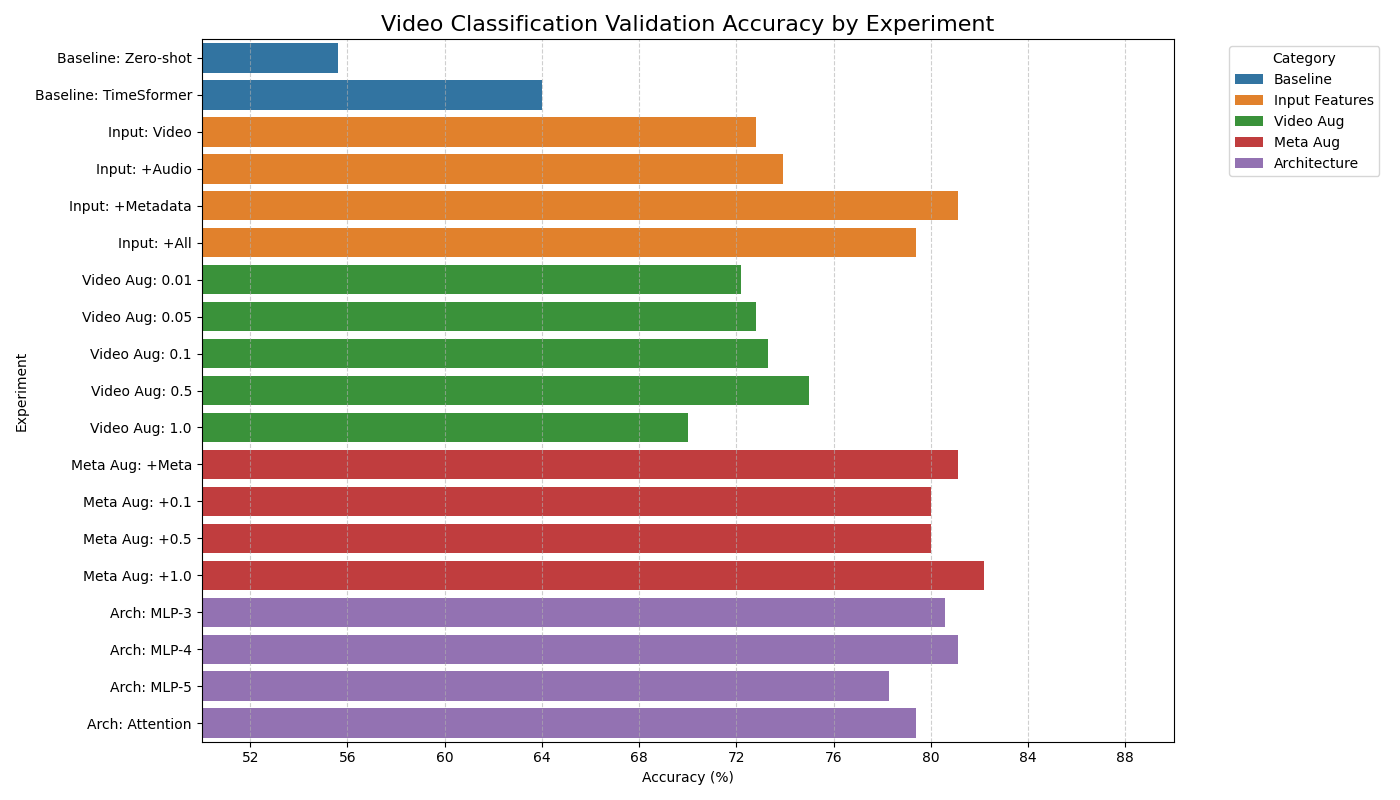
\includegraphics[width=0.8\linewidth]{asset/accuracy_plot.png} % Replace with actual image
% \end{center}
%    \caption{Summary of validation accuracy by experiment, showing progressive improvements.}
% \label{fig:summary_results}
% \end{figure}

% Placeholder for confusion matrix
\begin{figure}[t]
\begin{center}
% \fbox{\rule{0pt}{2in} \rule{0.9\linewidth}{0pt}}
   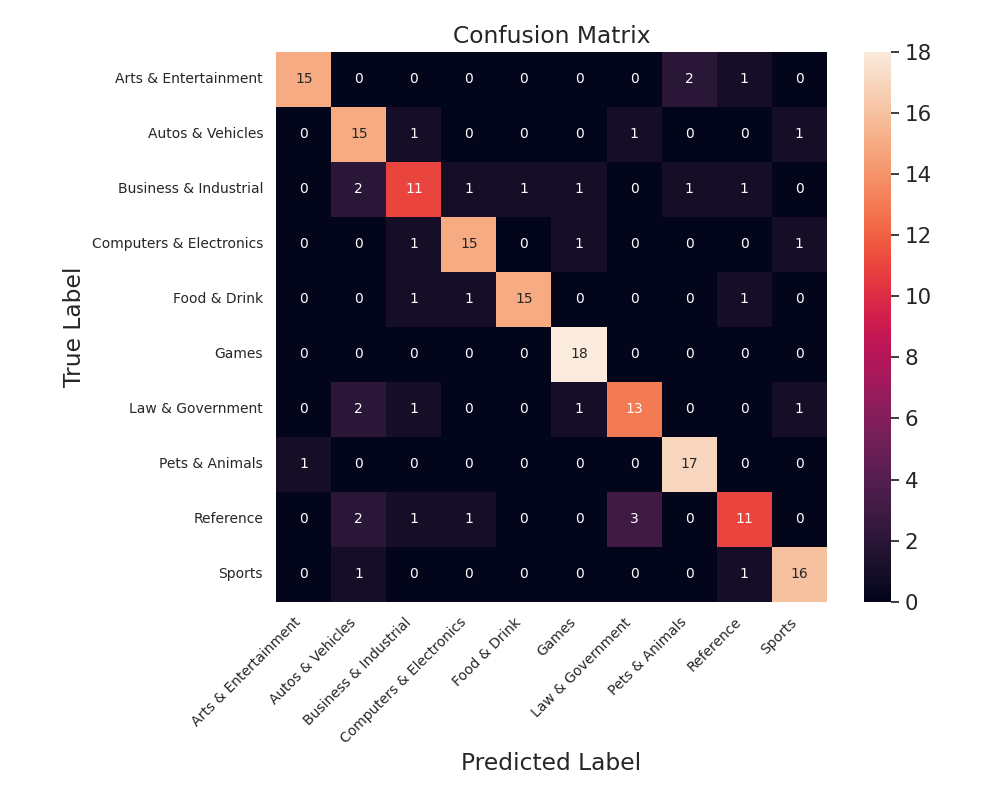
\includegraphics[width=0.8\linewidth]{asset/confusion_val.png} % Replace with actual image
\end{center}
   \caption{Confusion matrix of the 4 layers(MLP) model on the test set.}
\label{fig:confusion_matrix}
\end{figure}

%Our method achieves a compelling balance of high accuracy and drastically reduced training time, around 1 minute, compared to traditional complex models like 10 hours for TimeSformer fine-tuning.

The proposed methodology successfully achieves a compelling balance of high accuracy and significantly reduced training time, in comparison to conventional complex models such as TimeSformer fine-tuning, which can required up to ten hours.